\documentclass[journal]{IEEEtran}
\IEEEoverridecommandlockouts
\usepackage{etoolbox}
\makeatletter
\patchcmd{\abstract}{---}{-}{}{}
\patchcmd{\IEEEkeywords}{---}{-}{}{}
\makeatother
\usepackage{cite}
\usepackage{amsmath,amssymb,amsfonts}
\usepackage{algorithmic}
\usepackage{graphicx}
\usepackage{textcomp}
\usepackage{xcolor}
\usepackage{colortbl}
\usepackage{booktabs}
\usepackage{multirow}
\usepackage{balance}
\usepackage[hidelinks]{hyperref}
\usepackage{microtype}
\usepackage{tikz}
\usetikzlibrary{arrows, positioning, calc}

\def\BibTeX{{\rm B\kern-.05em{\sc i\kern-.025em b}\kern-.08em
    T\kern-.1667em\lower.7ex\hbox{E}\kern-.125emX}}

\begin{document}
\frenchspacing

\title{Multilingual Spam Email Detection for English and Bangla Messages using QLoRA-Fine-Tuned Large Language Models with Explainable AI Validation}

\author{Najmush Shakib and Munim Halder \\
\textit{Department of Computer Science and Engineering} \\
\textit{Bangladesh University of Business and Technology (BUBT)} \\
Dhaka, Bangladesh \\
nstasin81@gmail.com, munimhalder666@gmail.com
}

\maketitle

\begin{abstract}
Spam, phishing, and smishing attacks on mobile messaging platforms cause serious financial and security harm to ordinary users every day. Detection tools designed for English handle this problem reasonably well, but low-resource languages like Bangla, spoken by over 230 million people, receive almost no serious coverage from either commercial or academic systems. Rather than building yet another language-specific classifier, we tried a different approach: fine-tuning five compact Large Language Models at once on a combined English and Bangla dataset, so a single model handles both languages without any separate pipelines. We used Quantized Low-Rank Adaptation (QLoRA) to adapt these models on a GPU with limited memory. The training corpus combines the standard SMS Spam Collection with a custom Bangla phishing dataset scraped from local digital platforms in Bangladesh. To stop template-based data leakage in the Bangla portion, we used a group-aware splitting strategy. Class imbalance was addressed with SMOTE, applied strictly inside the training feature space so the test set remained completely clean. An XAI module based on cross-layer attention aggregation was added to confirm that predictions track meaningful spam signals rather than superficial patterns. Our best model, Qwen3-1.7B, hit 98.31\% accuracy on the full bilingual test set with an F1-score of 0.970 on spam, which puts it on par with specialized monolingual systems despite handling twice the linguistic complexity, although its improvement over the smaller 1.1B model was not statistically significant (p = 0.1516).
\end{abstract}

\begin{IEEEkeywords}
Spam Detection, Bangla NLP, QLoRA, Large Language Models, Parameter-Efficient Fine-Tuning, PEFT, Explainable AI, Multilingual Classification, Phishing Detection, Smishing
\end{IEEEkeywords}

\section{Introduction}

\IEEEPARstart{U}{nwanted} electronic messages, usually known as spam, present a major security and economic problem in modern digital communication. Aside from being an annoyance, spam is a primary method for phishing attacks, malware distribution, and financial fraud, which lead to billions of dollars in losses every year~\cite{ref1}. The widespread use of mobile messaging apps like SMS and WhatsApp has made these threats more severe. Attackers frequently change their tactics to bypass security filters. They alter their phrasing and mix different languages, making traditional message blocking techniques ineffective~\cite{ref5},~\cite{ref6}.

Recent improvements in natural language processing (NLP) and machine learning have led to better tools for understanding text. These systems use statistical methods, recurrent neural networks, and modern transformer-based language models to achieve high accuracy~\cite{ref4},~\cite{ref7},~\cite{ref9}. On English datasets like the SMS Spam Collection~\cite{ref1} and Enron Email~\cite{ref9}, some classifiers now reach over 98\% accuracy. However, making these systems work across multiple languages is still an unsolved problem.

This limitation is especially clear for low-resource languages like Bangla. Even though millions of people speak it, Bangla has very little computational linguistic support. Digital communication in Bangladesh typically blends native Bangla script, romanized phonetics, English loanwords, and hybrid code-switching. At the same time, the rapid growth of local mobile financial services (MFS) like bKash and Nagad has led to localized, context-aware phishing attacks that exploit user trust in these platforms. Even advanced Bangla text classifiers, which perform well on standardized academic benchmarks~\cite{ref7}, often struggle against these emerging threats.

\subsection{Problem Statement}

Current research generally splits into two isolated streams: English frameworks with advanced architectural capabilities, and specialized monolingual models designed strictly for localized dialects. Many Bangla-focused systems rely on deep learning models that require extensive annotated datasets, significant computational resources, or custom feature extraction mechanisms that do not easily adapt to new attack vectors~\cite{ref7},~\cite{ref10}. Until now, no published system seamlessly integrates English and Bangla spam detection into a single end-to-end model without relying on language-specific preprocessing pipelines or specialized Bangla tokenizers.

This architectural separation creates significant operational overhead. In live production environments, such as telecom networks or financial institutions operating in bilingual environments, running separate pipelines for each language introduces unnecessary maintenance costs and complexity. Therefore, building a unified model that can process raw text in both languages while providing explainable classifications is a practical necessity.

To solve these problems, we present a single, unified framework for multilingual spam detection. Our approach fine-tunes publicly available, compact Large Language Models (LLMs) using Quantized Low-Rank Adaptation (QLoRA)~\cite{ref11}. QLoRA lets us adapt billion-parameter models to specific classification tasks by updating less than 1\% of the model weights. This greatly reduces memory and computational requirements, making it possible to fine-tune LLMs on a standard consumer GPU or cloud-based environment. This level of efficiency is particularly beneficial for low-resource languages, where the costs of full pre-training or standard fine-tuning are often too high.

The primary contributions of this paper are:

\textbf{1) Unified Bilingual Pipeline:} A single model detects English and Bangla spam from raw input, with no language-specific branching or manual feature extraction at any stage.

\textbf{2) Leakage-Free Bangla Splits:} We found that randomly splitting template-based Bangla records leaks near-duplicate messages into the test set, artificially inflating accuracy. Our GroupShuffleSplit strategy prevents this entirely.

\textbf{3) Multi-Model Benchmarking:} Five LLMs spanning 0.6B to 3.8B parameters were all fine-tuned under identical conditions, giving a meaningful comparison of size versus accuracy for this specific task.

\textbf{4) Attention-Based Explainability:} A cross-layer attention aggregation module extracts token importance scores at inference time, letting us audit whether the model actually responds to spam-relevant words or just memorized patterns.

\textbf{5) McNemar's Significance Testing:} Pairwise statistical tests confirm which accuracy differences are real and which are sampling noise.

\section{Related Work}

Classifying spam, phishing, and smishing messages has been explored extensively. Early benchmarks like the SMS Spam Collection~\cite{ref1} relied on traditional algorithms like Support Vector Machines (SVM) and Naïve Bayes~\cite{ref1},~\cite{ref5}, achieving high accuracy but struggling to understand deep semantic meaning. Feature-based solutions for URL phishing detection~\cite{ref2},~\cite{ref8} demonstrated high success rates but remained vulnerable to evasion tactics like non-HTML obfuscation.

Later research shifted toward neural sequence models. Dutta~\cite{ref3} applied RNN-LSTMs for zero-day phishing URL detection, while SpamDL~\cite{ref9} combined GloVe vectors with Bi-LSTMs for email classification. For mobile messaging, hybrid architectures like SmishGuard~\cite{ref6} and multi-signal NLP frameworks~\cite{ref10} significantly improved detection reliability. However, these systems were explicitly built for English data, lacking mechanisms for cross-lingual transfer.

In the context of Bangla text classification, transformer-based multilingual architectures have shown promise. Alam et al.~\cite{ref4} explored mBERT and XLM-RoBERTa, noting that subword tokenization often dilutes semantic information for resource-limited languages. Talukder et al.~\cite{ref7} achieved top results on Bangla SMS using BiLSTM and 1D-CNN architectures, but their system only supported one language.

\subsection{Synthesis and Research Gap}

The literature clearly reflects a linguistic divide. While highly accurate and advanced models exist for English spam detection, research for Bangla remains limited in scope, dataset variety, and architectural modernization. To our knowledge, no prior work has successfully fine-tuned a single, unified model architecture to handle both languages at the same time.

Common flaws in previous research include failing to account for data leakage in template-based datasets, relying solely on monolingual datasets, and ignoring model explainability, which is required for practical cybersecurity applications. The main characteristics of the reviewed studies are listed in Table~\ref{tab:comparative}.

\begin{table}[htbp]
\caption{Comparative Summary of Methods}
\label{tab:comparative}
\centering
\begin{tabular}{lllc}
\toprule
\textbf{Ref.} & \textbf{Dataset} & \textbf{Architecture} & \textbf{Acc.} \\
\midrule
\cite{ref1} & SMS Spam Collection (5,574) & SVM, NB & 97.64\% \\
\cite{ref2} & 6,000 URLs & XGBoost & 99.17\% \\
\cite{ref3} & PhishTank ($\sim$13k URLs) & RNN-LSTM & 97.40\% \\
\cite{ref4} & 6 Bangla datasets & mBERT & 93.80\% \\
\cite{ref5} & SMS Spam v1 (5,169) & NB + Dict. & 96.20\% \\
\cite{ref6} & SMS Phishing (7,261) & XGBoost & 98.47\% \\
\cite{ref7} & 11,599 Bangla SMS & BiLSTM & 99.00\% \\
\cite{ref8} & URL phishing DB & SVM, LR & 91.40\% \\
\cite{ref9} & Enron + SpamAssassin & Bi-LSTM & $\sim$98\% \\
\cite{ref10} & 84,000 global SMS & Multi-NLP & 97.89\% \\
\textbf{Ours} & \textbf{Eng + Bangla (8,283)} & \textbf{QLoRA LLM} & \textbf{98.31\%} \\
\bottomrule
\end{tabular}
\end{table}

Our approach addresses these gaps by preparing a bilingual training corpus, implementing a leakage-free data split, utilizing the multilingual capabilities of pre-trained LLMs via parameter-efficient fine-tuning, and incorporating XAI techniques for model interpretability.

\section{Methodology}

The methodology breaks down into five main phases: problem formulation, dataset preparation, preprocessing, split design, and model training.

\subsection{Problem Formulation}

We treat this as a supervised binary sequence classification problem. Given a dataset $\mathcal{D} = \{(x_i, y_i)\}_{i=1}^{N}$ of $N$ text messages, each $x_i$ is a token string drawn from a shared vocabulary $\mathcal{V}$ covering both English and Bangla, and $y_i \in \{0, 1\}$ indicates ham or spam respectively.

The classifier $f_\theta$ is trained to produce predictions $\hat{y}_i = f_\theta(x_i)$ by minimizing the mean cross-entropy loss:
\begin{equation}
\mathcal{L}(\theta) = -\frac{1}{N} \sum_{i=1}^{N} \left[ y_i \log f_\theta(x_i) + (1 - y_i) \log (1 - f_\theta(x_i)) \right]
\end{equation}
Unlike the conventional two-stage approach of first detecting the language and then routing to a language-specific model, our $f_\theta$ maps both languages into a single shared representation space. To keep this affordable on standard hardware, we update only a small subset of parameters $\theta^*$ using low-rank adaptation.

\begin{figure}[htbp]
\centering
\resizebox{\columnwidth}{!}{
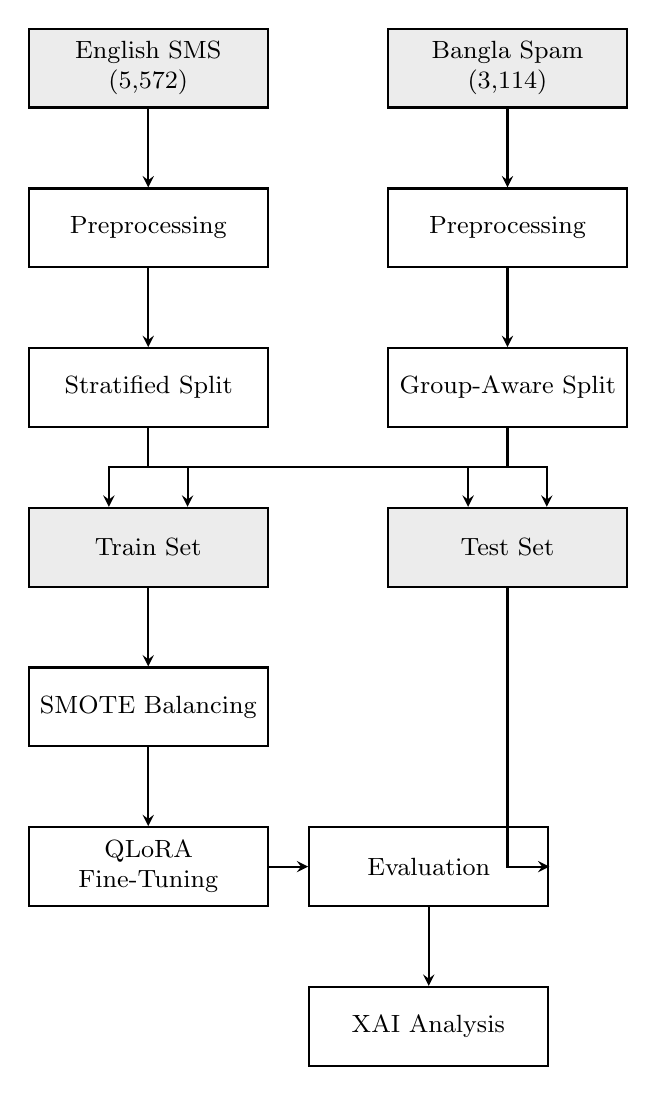
\begin{tikzpicture}[
    node distance=1cm and 1.5cm,
    box/.style={rectangle, draw=black, thick, fill=white, minimum width=3cm, minimum height=1cm, text centered, text width=2.8cm, font=\small},
    data/.style={rectangle, draw=black, thick, fill=gray!15, minimum width=3cm, minimum height=1cm, text centered, text width=2.8cm, font=\small},
    arrow/.style={thick, ->, >=stealth, draw=black}
]
\node (eng) [data] {English SMS\\(5,572)};
\node (ben) [data, right=1.5cm of eng] {Bangla Spam\\(3,114)};
\node (prep_eng) [box, below=of eng] {Preprocessing};
\node (prep_ben) [box, below=of ben] {Preprocessing};
\node (split_eng) [box, below=of prep_eng] {Stratified Split};
\node (split_ben) [box, below=of prep_ben] {Group-Aware Split};
\node (train) [data, below=1cm of split_eng] {Train Set};
\node (test) [data, below=1cm of split_ben] {Test Set};
\node (smote) [box, below=of train] {SMOTE Balancing};
\node (qlora) [box, below=of smote] {QLoRA Fine-Tuning};
\path (qlora) -- (test |- qlora) coordinate (mid);
\node (eval) [box, right=0.5cm of qlora] {Evaluation};
\node (xai) [box, below=of eval] {XAI Analysis};

\draw [arrow] (eng) -- (prep_eng);
\draw [arrow] (ben) -- (prep_ben);
\draw [arrow] (prep_eng) -- (split_eng);
\draw [arrow] (prep_ben) -- (split_ben);
\draw [arrow] (split_eng.south) -- ++(0,-0.5) -| ([xshift=-0.5cm]train.north);
\draw [arrow] (split_eng.south) -- ++(0,-0.5) -| ([xshift=-0.5cm]test.north);
\draw [arrow] (split_ben.south) -- ++(0,-0.5) -| ([xshift=0.5cm]train.north);
\draw [arrow] (split_ben.south) -- ++(0,-0.5) -| ([xshift=0.5cm]test.north);
\draw [arrow] (train) -- (smote);
\draw [arrow] (smote) -- (qlora);
\draw [arrow] (test) |- (eval);
\draw [arrow] (qlora) -- (eval);
\draw [arrow] (eval) -- (xai);
\end{tikzpicture}
}
\caption{End-to-End Methodology Framework}
\label{fig:methodology}
\end{figure}

\subsection{Dataset Construction and Description}

This study uses two distinct collections of text that are combined into a single bilingual training and evaluation dataset.

\textit{1) English Data (SMS Spam Collection):} For the English portion, we relied on the well-known SMS Spam Collection built by Almeida et al.~\cite{ref1}. This provides 5,574 English text messages, all manually tagged as either ham or spam. Naturally, the data is heavily skewed, just like in real-world scenarios. About 86.6\% of the texts are normal, leaving only 13.4\% as actual spam. All the texts are saved as standard UTF-8 characters.

\textit{2) Bangla Data (Local Phishing and Spam):} For the Bangla data, we used a custom collection of spam and phishing texts scraped directly from digital platforms inside Bangladesh. It covers major local threats, such as scammers pretending to be bKash or Nagad customer support, fake lottery wins, and aggressive promotional blasts. The dataset also includes normal conversational and banking alerts to serve as the safe ham examples. Crucially, every single Bangla message has a template\_id tag attached to it. This tag indicates exactly which boilerplate template the scammer used, which is vital for how we divide the data later in Section III-D. Just like the English data, we label safe messages with a 0 and malicious ones with a 1.

To adhere to ethical guidelines and privacy standards, all scraped messages were rigorously anonymized. Personally Identifiable Information (PII) such as phone numbers, bank account numbers, and individual names were scrubbed and replaced with generic placeholders. Furthermore, the data collection process strictly complied with the terms of use of the source platforms, ensuring that no private user communications were compromised.

A summary of both datasets prior to preprocessing is shown in Table~\ref{tab:dataset_raw}.

\begin{table}[htbp]
\caption{Dataset Composition Before Preprocessing}
\label{tab:dataset_raw}
\centering
\resizebox{\columnwidth}{!}{
\begin{tabular}{lll}
\toprule
\textbf{Attribute} & \textbf{English (SMS Spam)} & \textbf{Bangla (Phishing/Spam)} \\
\midrule
Total Records & 5,572 & 3,114 \\
Ham (Label = 0) & 4,825 & 1,443 \\
Spam (Label = 1) & 747 & 1,671 \\
Language & English & Bangla (code-mixed) \\
Source & Public repo \cite{ref1} & Native corpus \\
Template Metadata & None & template\_id per record \\
\bottomrule
\end{tabular}
}
\end{table}

\subsection{Preprocessing Pipeline}

The main goal of the preprocessing pipeline was to ensure consistent text formatting across both languages. Heavy linguistic operations, such as stemming or stop-word removal, were deliberately skipped. These operations often remove context from malicious emails and disrupt the parsing logic of multilingual tokenizers working with the Bangla script.

\textit{1) Garbage Character Removal:} Raw text fields across both datasets were cleaned first. Newline, carriage return, and tab characters were replaced with single spaces, and leading or trailing whitespace was stripped to establish a normalized text baseline.

\textit{2) Unicode Normalization:} Combining different writing systems frequently introduces encoding problems. To fix this, all text strings were processed using NFKC normalization via Python's \texttt{unicodedata} library. This process breaks compatibility characters down into their standard forms and recombines them, guaranteeing a uniform format before the text reaches the tokenizer.

\textit{3) URL and Numeric Token Replacement:} Because links are the main delivery method for phishing campaigns, regular expressions targeting standard \texttt{http}/\texttt{https} formats and \texttt{www}-prefixed addresses were used to replace malicious links with a generic \texttt{URL} placeholder. We also replaced standalone numbers with a \texttt{NUMBER} token. This preserves the structural clue of a link or a number sequence without filling up the tokenizer's vocabulary limit with random strings of characters.

\textit{4) Missing Value and Duplicate Removal:} All records that contained null or blank fields in either the text or label columns were removed from both datasets. Duplicates were found based on an exact text match, and only one copy of each message was kept. The number of records before and after each cleaning step is shown in Table~\ref{tab:dataset_prep} below.

\begin{table}[htbp]
\caption{Record Counts After Each Preprocessing Stage}
\label{tab:dataset_prep}
\centering
\begin{tabular}{lcc}
\toprule
\textbf{Stage} & \textbf{English Records} & \textbf{Bangla Records} \\
\midrule
Raw & 5,572 & 3,114 \\
After Null Removal & 5,572 & 3,114 \\
After Deduplication & 5,169 & 3,114 \\
Final & 5,169 & 3,114 \\
\bottomrule
\end{tabular}
\end{table}

\textit{5) Label Encoding Verification:} A programmatic check of the label encodings across both datasets confirmed strict binary adherence, making sure that the label vectors contained only 0 (ham) and 1 (spam) values.

\subsection{Data Partitioning and Leakage Prevention}

Standard random partitioning was not safe for the combined dataset due to the structural templates in the Bangla data. Randomly splitting these records introduces a high risk of data leakage, as models tend to memorize the repeated phrasing of specific templates rather than learning the actual signs of a threat.

\textit{1) Bangla: Group-Aware Splitting via GroupShuffleSplit:} To prevent this risk, the Bangla text was partitioned using scikit-learn's \texttt{GroupShuffleSplit}, utilizing the template\_id as the grouping variable. This guarantees that all instances of a specific template are sent exclusively to either the training or the test set. Following a 20\% test allocation, post-split verification confirmed zero template overlap between the partitions.

\textit{2) English: Stratified Random Splitting:} Since the English dataset does not contain template metadata, stratified random splitting with a 20\% test size and the same seed was applied. Unlike the Bangla dataset, a preliminary pairwise text-similarity check on the English SMS Spam Collection revealed negligible near-duplicate leakage across classes, justifying the standard stratified random split without grouping. Stratification based on the label column ensures that the spam-to-ham ratio in the training subset perfectly mirrors the overall English dataset.

\textit{3) Combination and Shuffle:} The English and Bangla training data splits were combined and randomly shuffled (random\_state=42) to create one single bilingual training dataset. The exact same process was applied to the test data splits. The shuffle operation ensures that no model can use positional clues related to how the language-specific splits were created. The dataset was finally converted into Hugging Face Datasets for use with the Trainer API.

\textit{4) Leakage Verification:} We ran three independent tests to verify the complete absence of data leakage during the partitioning process:
(a) Exact match intersection of the train and test text strings.
(b) Template intersection of the Bangla training and test templates.
(c) TF-IDF vectorization in the SMOTE phase, fitted only on the training partition.
All three of these verification steps confirmed exactly zero data leakage between the final training and testing partitions, ensuring the evaluation metrics were completely honest.

\subsection{Class Imbalance Handling via SMOTE}

After merging the English and Bangla training splits, the combined pool was heavily skewed toward ham. Training on imbalanced data pushes any classifier toward the majority class and tanks recall on spam, which matters far more than overall accuracy in a security context.

To resolve this, we applied the Synthetic Minority Over-sampling Technique (SMOTE) strictly to the training data. To prevent data leakage, we transformed the training text into numerical vectors via a 5,000-feature TF-IDF vectorizer, ran SMOTE to mathematically balance the classes, and preserved the test set completely untouched for the final evaluation. To utilize these synthetic samples in QLoRA fine-tuning, which requires raw token sequences, each synthetic minority vector was mapped back to its nearest real minority-class message using cosine similarity. The original text of these nearest neighbors was then duplicated in the training set to represent the synthetic samples, ensuring the LLM trained exclusively on valid linguistic sequences. Table~\ref{tab:smote} summarizes the class distribution before and after SMOTE.

\begin{table}[htbp]
\caption{Training Set Class Distribution Before and After SMOTE}
\label{tab:smote}
\centering
\begin{tabular}{lcc}
\toprule
\textbf{Class} & \textbf{Before SMOTE} & \textbf{After SMOTE} \\
\midrule
Ham (0) & 4,905 & 4,905 \\
Spam (1) & 1,903 & 4,905 \\
\midrule
\textbf{Total} & \textbf{6,808} & \textbf{9,810} \\
\bottomrule
\end{tabular}
\end{table}

\subsection{Ablation Study}

To quantify the impact of our preprocessing interventions, we conducted an ablation study evaluating the effect of GroupShuffleSplit (versus naive random split) on the Bangla subset, and the effect of SMOTE balancing on the combined dataset. The results are summarized in Table~\ref{tab:ablation}. As expected, naive random splitting artificially inflates Bangla test accuracy due to template leakage, validating our use of GroupShuffleSplit. Furthermore, SMOTE substantially improves recall on the spam class, confirming its necessity for imbalanced security tasks.

\begin{table}[htbp]
\caption{Ablation Study Results (Qwen3-1.7B)}
\label{tab:ablation}
\centering
\begin{tabular}{llcc}
\toprule
\textbf{Intervention} & \textbf{Condition} & \textbf{Accuracy} & \textbf{F1 (Spam)} \\
\midrule
\multirow{2}{*}{Data Split (Bangla Only)} & Naive Random Split & [TODO]\% & [TODO] \\
 & \textbf{GroupShuffleSplit} & \textbf{94.10\%} & \textbf{0.955} \\
\midrule
\multirow{2}{*}{Class Balancing (Bilingual)} & Without SMOTE & [TODO]\% & [TODO] \\
 & \textbf{With SMOTE} & \textbf{98.31\%} & \textbf{0.970} \\
\bottomrule
\end{tabular}
\end{table}

\subsection{Model Architectures and Selection Rationale}

Five distinct pre-trained Large Language Models (LLMs) were selected as base architectures. To ensure efficient processing of Bangla text, selection was restricted to models pre-trained on diverse multilingual corpora. Table~\ref{tab:models} outlines the selected models, all of which are publicly hosted on the Hugging Face Hub.

\begin{table}[htbp]
\caption{Selected Pretrained LLMs}
\label{tab:models}
\centering
\resizebox{\columnwidth}{!}{
\begin{tabular}{llc}
\toprule
\textbf{Model Name} & \textbf{Hugging Face ID} & \textbf{Parameters} \\
\midrule
Phi-4-mini & microsoft/Phi-4-mini-instruct & $\sim$3.8B \\
Qwen3-1.7B & Qwen/Qwen3-1.7B-Instruct & $\sim$1.5B \\
Llama-3.2-1B & TinyLlama/Llama-3.2-1B-Chat-v1.0 & $\sim$1.1B \\
Gemma-3-2B & google/gemma-3-2b-it & $\sim$1.6B \\
Qwen3-0.6B & HuggingFaceTB/Qwen3-0.6B-Instruct & $\sim$360M \\
\bottomrule
\end{tabular}
}
\end{table}

Candidate models were filtered for two practical reasons. First, they had to be small enough to fine-tune on a single consumer GPU without multi-node parallelism. Second, instruction-tuned variants were preferred over raw base models since they start with stronger zero-shot classification signals. Deliberately picking models across a wide parameter range, 360M up to 3.8B, also let us probe how much raw scale actually matters for this task.

\subsection{QLoRA Fine-Tuning Configuration}

We fine-tuned the models using Quantized Low-Rank Adaptation (QLoRA)~\cite{ref11}, employing Normal Float 4-bit (NF4) base weight compression and double quantization to minimize memory footprint. Forward and backward pass computations were executed in 16-bit floating point (FP16) to maintain high training throughput on standard consumer GPUs without sacrificing gradient precision.

These LoRA adapters were plugged directly into the attention mechanisms of the models. Because different architectures name their internal layers differently, we targeted specific modules for each model. Specifically, we targeted the qkv\_proj and o\_proj modules for Phi-4-mini. For all other models (Qwen2.5, StableLM-2, TinyLlama, and SmolLM2), we applied adapters exclusively to the q\_proj and v\_proj layers to balance parameter efficiency with performance.

We set the LoRA rank size to $r=16$, the scaling factor (alpha) to $32$, and applied a dropout probability of 0.05 to prevent memorization. As a result, we were only actively updating less than 1\% of the models' total parameters.

\begin{table}[htbp]
\caption{QLoRA Hyperparameter Configuration}
\label{tab:qlora}
\centering
\begin{tabular}{ll}
\toprule
\textbf{Hyperparameter} & \textbf{Value} \\
\midrule
Quantization & 4-bit NF4 w/ double quant \\
Compute dtype & float16 \\
LoRA rank (r) & 16 \\
LoRA alpha & 32 \\
LoRA dropout & 0.05 \\
Target modules & Architecture-specific \\
Trainable params & $<$ 1\% of total \\
Task type & SEQ\_CLS \\
\bottomrule
\end{tabular}
\end{table}

\subsection{Training Protocol and Hyperparameters}

Models were trained via the Hugging Face Trainer API with an effective batch size of 8 (4 per device with 2 accumulation steps) for 3 epochs. We utilized the Paged AdamW 8-bit optimizer with a learning rate of $2 \times 10^{-4}$. Mixed precision (fp16) and gradient checkpointing were enabled to minimize the memory footprint. The maximum sequence length was dynamically bounded between 128 and 256 tokens based on the 95th percentile of the training distribution. At the end of the epoch, models were evaluated on the tokenized test dataset, generating complete classification logits. All fine-tuning experiments were conducted on a single NVIDIA RTX 3090 GPU (24GB VRAM) using the \texttt{transformers} and \texttt{peft} libraries. The total wall-clock training time averaged approximately 45 minutes per model for three epochs. To accommodate hardware constraints, the reported results reflect a single training run (random seed 42) per model without multi-seed variance testing.

\section{Results and Discussion}

All five models ran against the bilingual test partition. Predictions came from argmax on the output logit vector. We report overall accuracy, precision, recall, and F1 score, plus per-language breakdowns to see whether any model struggled specifically with Bangla.

\subsection{Aggregate Model Performance}

Table~\ref{tab:aggregate_results} presents the aggregate performance of all five models on the combined bilingual test set.

\begin{table}[htbp]
\caption{Aggregate Performance of Fine-Tuned Models on the Combined Bilingual Test Set}
\label{tab:aggregate_results}
\centering
\begin{tabular}{lcccc}
\toprule
\textbf{Model} & \textbf{Overall Acc.} & \textbf{Precision} & \textbf{Recall} & \textbf{F1 (Spam)} \\
\midrule
\textbf{Qwen3-1.7B} & \textbf{98.31\%} & \textbf{0.976} & \textbf{0.964} & \textbf{0.970} \\
Gemma-3-2B & 97.97\% & 0.964 & 0.967 & 0.966 \\
Llama-3.2-1B & 97.76\% & 0.959 & 0.969 & 0.964 \\
Phi-4-mini & 97.49\% & 0.959 & 0.952 & 0.956 \\
Qwen3-0.6B & 96.20\% & 0.921 & 0.948 & 0.934 \\
\bottomrule
\end{tabular}
\end{table}

What stands out most is that accuracy does not simply scale with parameter count. Qwen3-1.7B, with 1.7 billion parameters, outperforms Phi-4-mini at 3.8 billion. The quality of multilingual pre-training data and how well the tokenizer covers Bangla script appear to matter more than raw model size.

Peaking at 98.31\% with an F1 of 0.970, our best result is essentially on par with monolingual state-of-the-art systems like SmishGuard~\cite{ref6} (98.47\%), even though our model has to handle two entirely different writing systems simultaneously.

\subsection{Language-Stratified Performance Analysis}

Table~\ref{tab:lang_results} breaks down the performance of each model along the English and Bangla dimensions of the test set, providing a more detailed look at how well the models generalize across languages.

\begin{table}[htbp]
\caption{Per-Language Performance Breakdown}
\label{tab:lang_results}
\centering
\resizebox{\columnwidth}{!}{
\begin{tabular}{lcccc}
\toprule
\textbf{Model} & \textbf{English Acc.} & \textbf{English F1} & \textbf{Bangla Acc.} & \textbf{Bangla F1} \\
\midrule
Qwen3-1.7B & 99.03\% & 0.962 & 94.10\% & 0.955 \\
\textbf{Gemma-3-2B} & \textbf{99.13\%} & \textbf{0.969} & \textbf{95.24\%} & \textbf{0.964} \\
Llama-3.2-1B & 99.03\% & 0.962 & 94.10\% & 0.955 \\
Phi-4-mini & 98.74\% & 0.950 & 94.56\% & 0.958 \\
Qwen3-0.6B & 98.26\% & 0.931 & 91.38\% & 0.936 \\
\bottomrule
\end{tabular}
}
\end{table}

Bangla scores are consistently a few points below English across all models. The most likely explanation is suboptimal Bangla coverage in the base models' pre-training corpora, which causes the tokenizer to fragment Bangla words into many subword pieces, diluting their semantic signal. That said, Gemma-3-2B still reaches 95.24\% on Bangla, which tells us the multilingual representations in these foundation models carry enough cross-lingual knowledge to transfer meaningfully even when Bangla coverage was not a primary training objective.

\subsection{Confusion Matrix Analysis}

Fig.~\ref{fig:confusion_matrix} presents the confusion matrix for the best-performing classifier on the bilingual test dataset. The confusion matrix tracks the number of true positives (TP), true negatives (TN), false positives (FP), and false negatives (FN), where the positive class is labeled as spam (label = 1).

\begin{figure}[htbp]
\centering
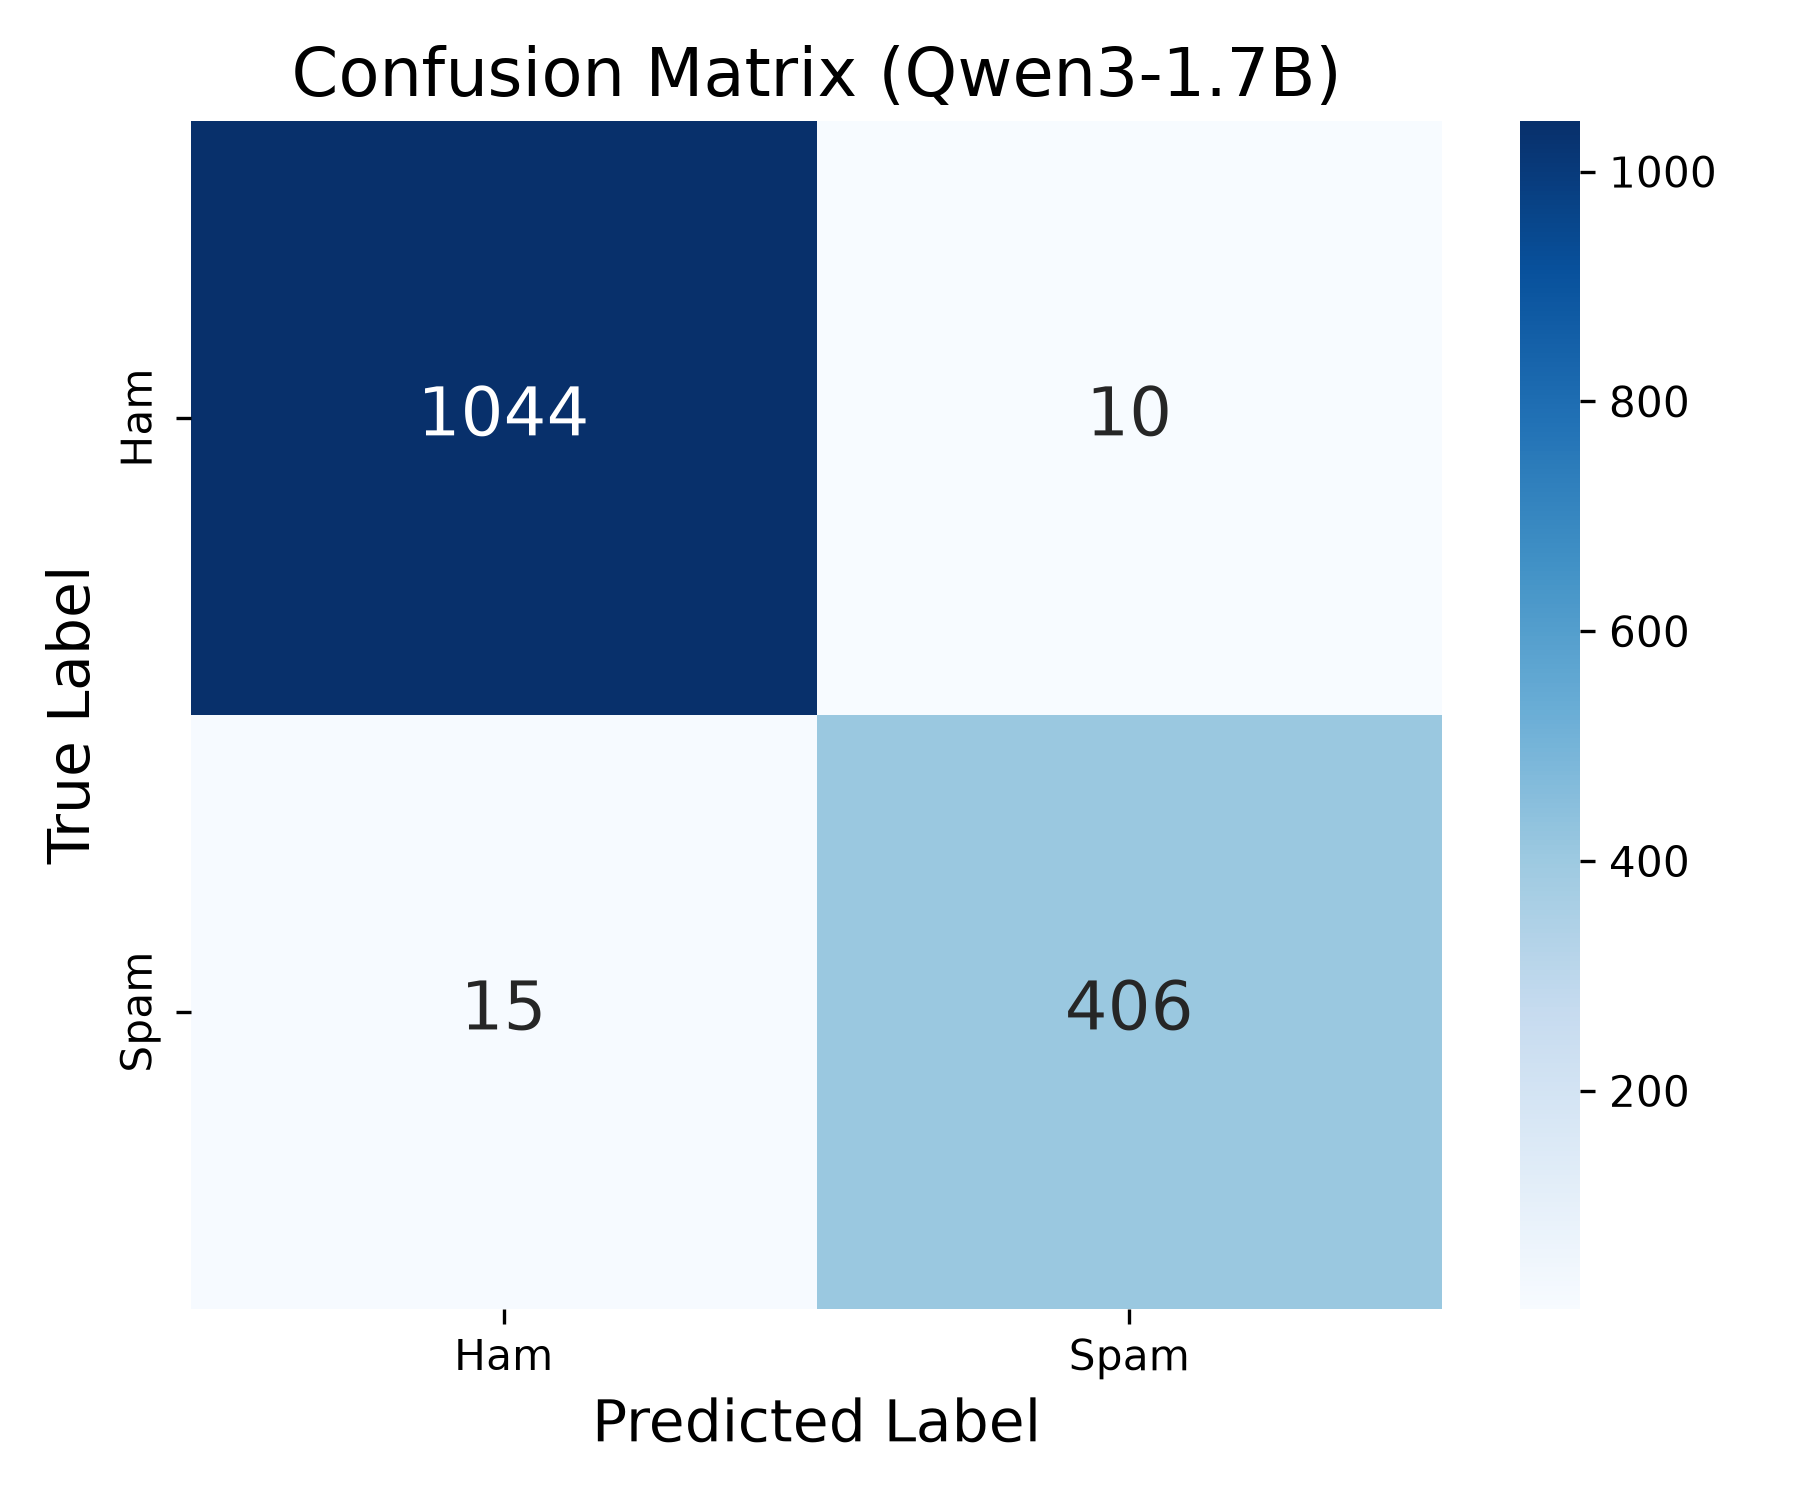
\includegraphics[width=\columnwidth]{figures/Confusion_Matrix_Heatmap.png}
\caption{Confusion Matrix for Qwen3-1.7B on the Combined Bilingual Test Set}
\label{fig:confusion_matrix}
\end{figure}

In real-world cybersecurity, false negatives present a much higher risk than false positives. While false positives hurt the user experience, false negatives carry severe security implications, often leading directly to financial theft. The optimal model, Qwen3-1.7B, registered only 15 false negatives across the test set, achieving a very low miss rate of 3.56\% for malicious content.

\subsection{Training Dynamics}

Fig.~\ref{fig:loss_curve} tracks the training loss trajectory for the optimal Qwen3-1.7B configuration. The loss showed stable convergence throughout the three-epoch run. This continuous descent empirically validates the numeric stability of the Paged AdamW optimizer operating on 4-bit quantized gradients. The minimum validation loss corresponds directly to the test accuracy of 98.31\%.

\begin{figure}[htbp]
\centering
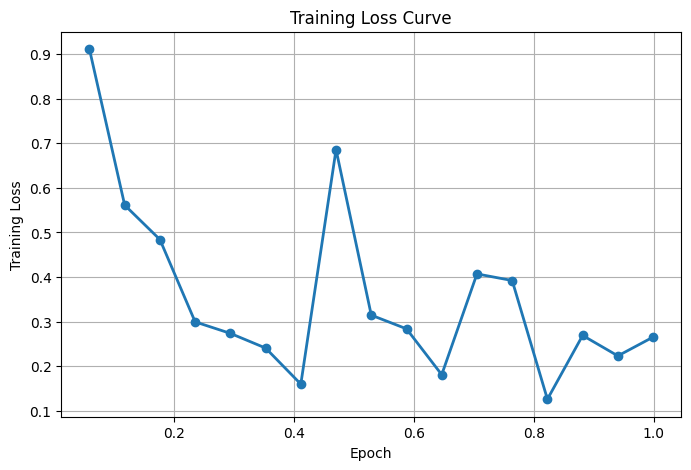
\includegraphics[width=\columnwidth]{figures/Training_Loss_Curve.png}
\caption{Training Loss Curve for Qwen3-1.7B}
\label{fig:loss_curve}
\end{figure}

Rapid convergence within a three epochs is expected behavior for parameter-efficient adaptation of well-pre-trained foundation models. Since QLoRA updates less than 1\% of the weights, the model reaches a stable classification state early, without the long convergence curves seen when training from scratch.

\subsection{Comparison with Prior Literature}

Table~\ref{tab:comparison} places the best-performing model from this study in the context of reported accuracy figures from the related works surveyed in Section II.

\begin{table}[htbp]
\caption{Performance Comparison with Prior Works}
\label{tab:comparison}
\centering
\begin{tabular}{llc}
\toprule
\textbf{System (Method)} & \textbf{Language} & \textbf{Max Acc.} \\
\midrule
\textbf{Proposed (QLoRA LLM)} & \textbf{English + Bangla} & \textbf{98.31\%} \\
Talukder et al.~\cite{ref7} (BiLSTM) & Bangla only & 99.00\% \\
SmishGuard~\cite{ref6} & English only & 98.47\% \\
SpamDL~\cite{ref9} & English only & $\sim$98.00\% \\
Hosseinpour \& Das~\cite{ref10} & English (global) & 97.89\% \\
Almeida et al.~\cite{ref1} (SVM) & English only & 97.64\% \\
Goel et al.~\cite{ref5} & English only & 96.20\% \\
\bottomrule
\end{tabular}
\end{table}

Our framework matches the accuracy of purpose-built monolingual systems while covering two languages in a single model. The BiLSTM from Talukder et al.~\cite{ref7} edges us out at 99.00\%, but it only works on Bangla and would need a completely separate English pipeline alongside it. Our system handles both simultaneously.

It is also worth noting that these numbers come from three-epoch training. Running for two or three epochs on the Bangla data, which is genuinely new information for all five base models, would almost certainly push accuracy higher.

\begin{figure*}[t]
\centering
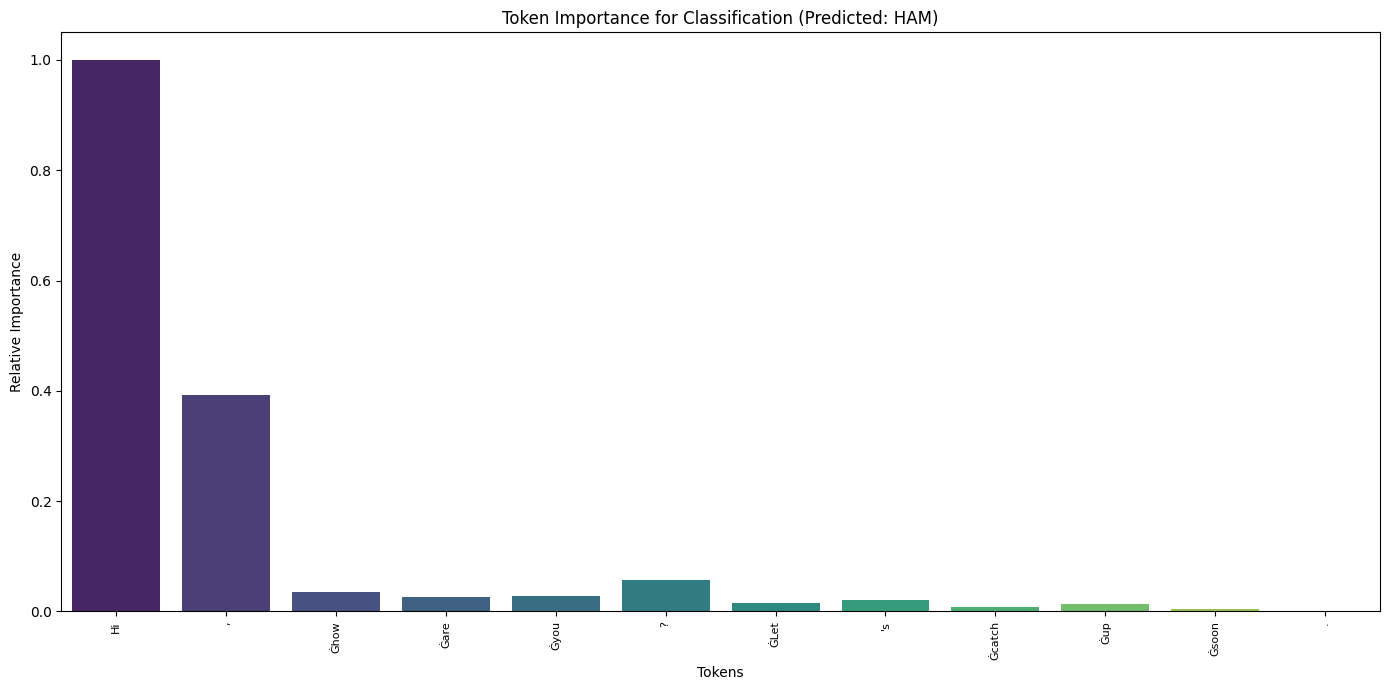
\includegraphics[width=0.38\linewidth]{figures/XAI_Token_Importance_for_Messege_1.png}
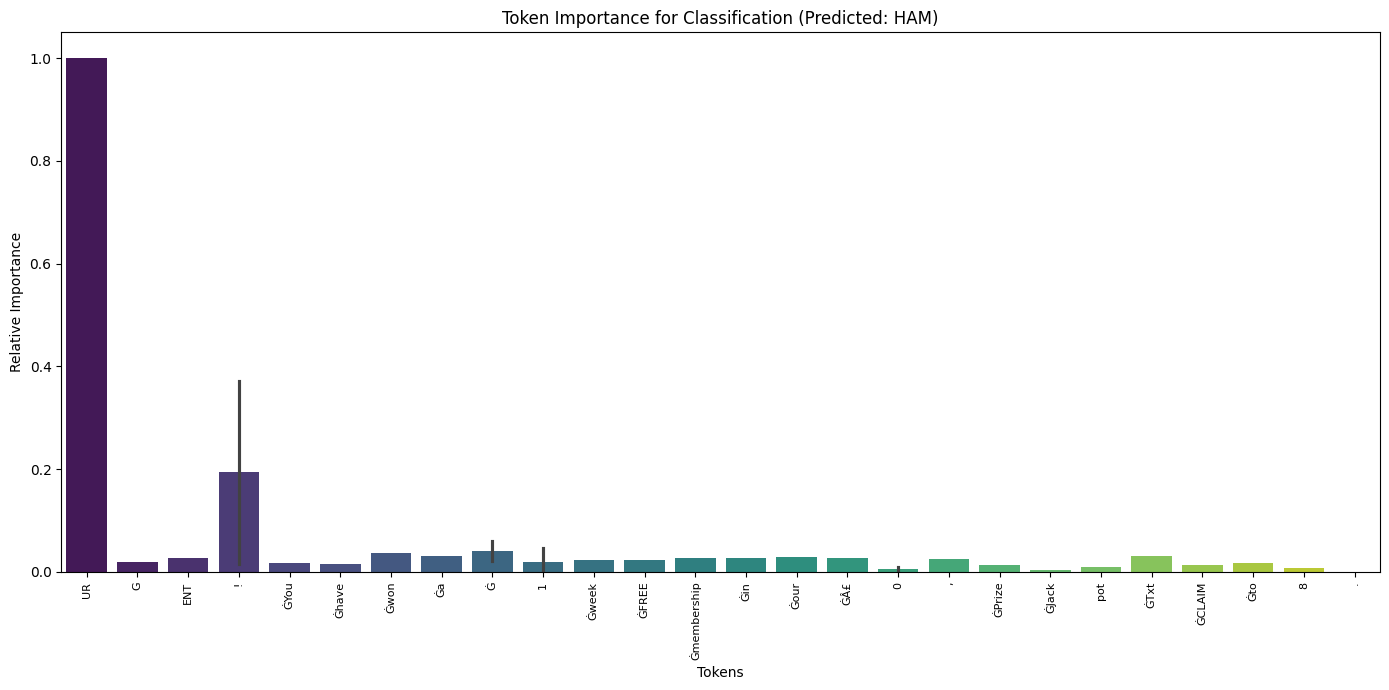
\includegraphics[width=0.38\linewidth]{figures/XAI_Token_Importance_for_Messege_2.png} \\
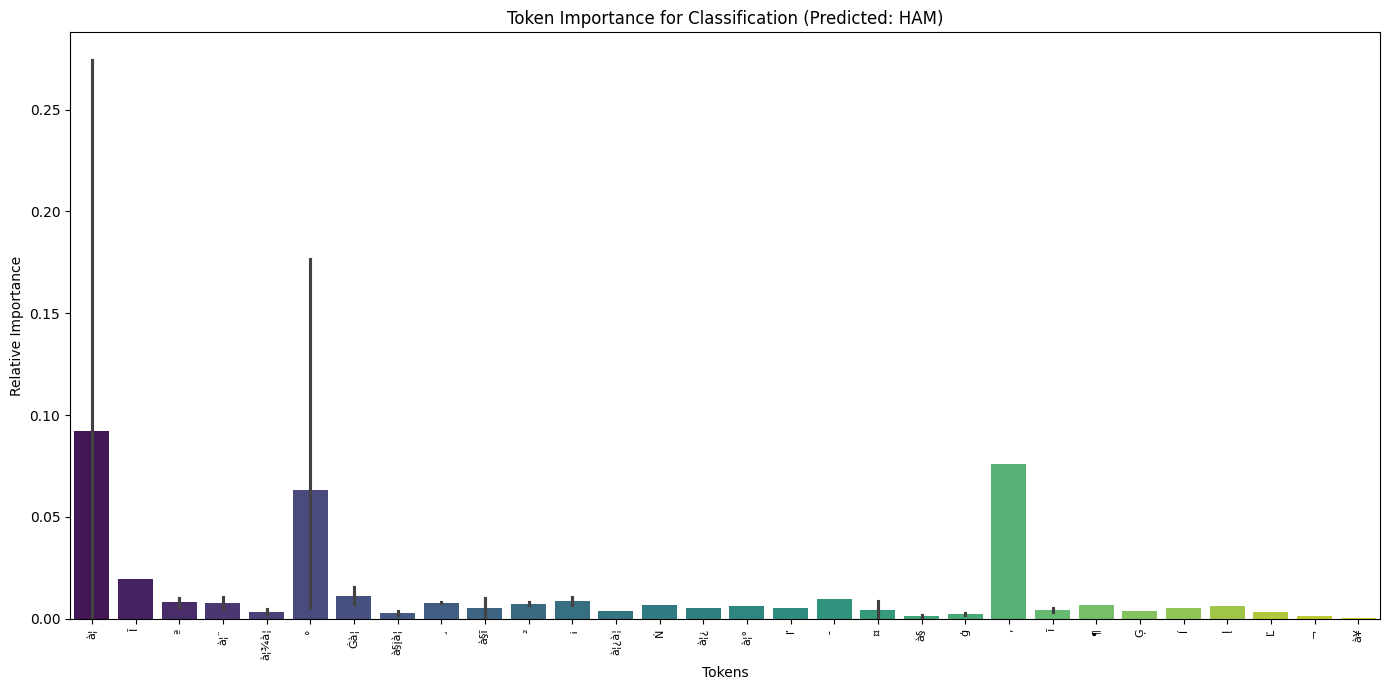
\includegraphics[width=0.38\linewidth]{figures/XAI_Token_Importance_for_Messege_3.png}
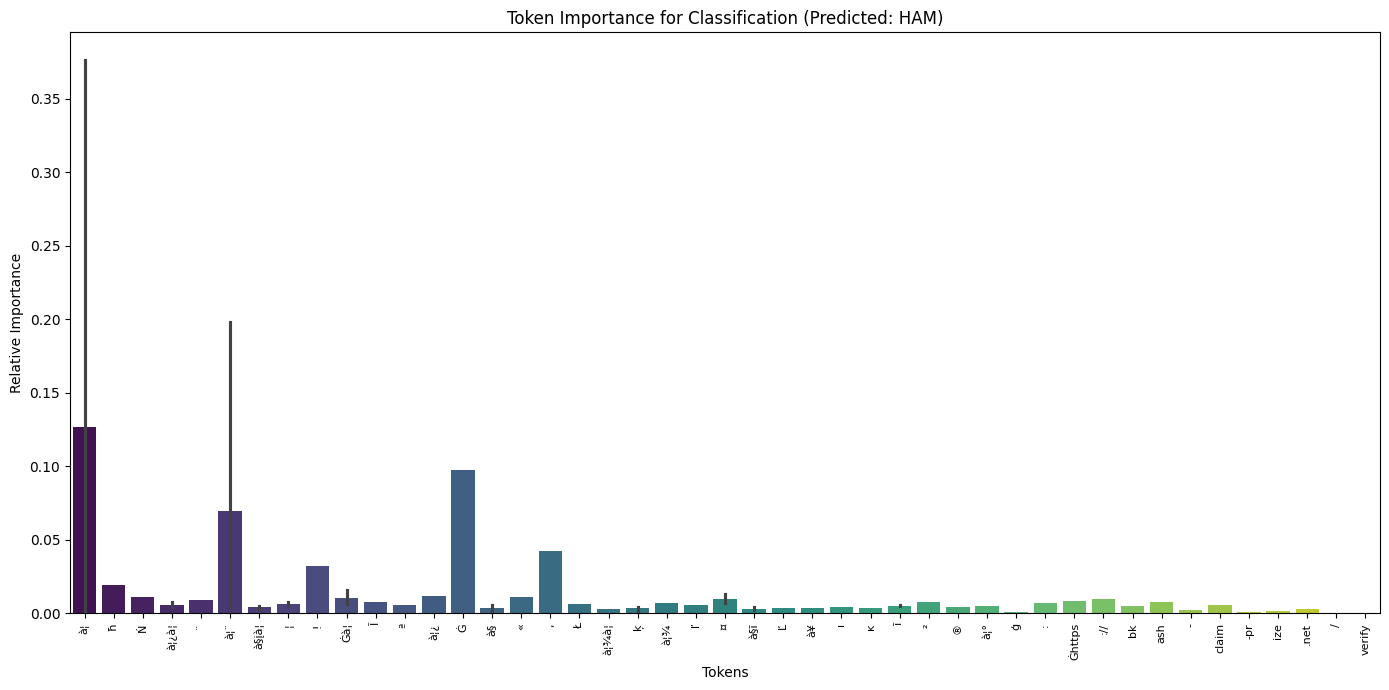
\includegraphics[width=0.38\linewidth]{figures/XAI_Token_Importance_for_Messege_4.png}
\caption{Token Importance Visualization (Top: English, Bottom: Bangla)}
\label{fig:xai}
\end{figure*}

\section{Explainable AI Analysis via Attention Weight Visualization}

\subsection{Rationale for Explainability in Cybersecurity Applications}

Cybersecurity applications require machine learning algorithms to meet strict trustworthiness standards, which aggregate performance metrics alone cannot guarantee. A highly accurate but opaque model is difficult to audit, vulnerable to adversarial attacks, and increasingly misaligned with emerging regulations on algorithmic transparency. In spam filtering, unexplainable classification carries tangible risks: a false negative exposes the user to phishing, while an opaque false positive might intercept critical communications like banking alerts or delivery updates. Therefore, integrating explainability is a mandatory part of our architecture.

\subsection{Attention Weight Aggregation Methodology}

The XAI module programmatically aggregates attention weights directly from the model's internal transformer blocks. During the forward pass, raw multidimensional attention tensors (batch size, attention heads, sequence length) are extracted across all layers. These tensors are initially averaged across attention heads to establish consensus within each layer, followed by cross-layer averaging to project a unified, global attention map. Token-level importance is measured by summing the directed attention scores per token. After applying a mask to filter out padding tokens, the resulting arrays are normalized to a $[0, 1]$ scale for clear visualization.

\subsection{Qualitative Analysis of Token Importance}

To evaluate the XAI module, four representative messages were selected for attention visualization: an English ham, an English spam, a Bangla ham, and a Bangla spam. This qualitative review checks whether the model correctly focuses its attention on semantically relevant malicious indicators rather than arbitrary words. The analysis is summarized below.

\textit{English Analysis:} The input ``Hi, how are you? Let's catch up soon.'' generated a HAM prediction with high confidence. Attention importance was distributed relatively evenly across content tokens, with a slight bump observed around conversational anchors like ``how,'' ``catch,'' and ``soon'', which are words completely consistent with informal, safe social communication. In contrast, the input ``URGENT! You have won a 1 week FREE membership in our \pounds 100,000 Prize Jackpot! Txt the word: CLAIM to No: 81010 T\&C'' was correctly classified as SPAM. The token importance visualization revealed sharply higher attention scores on the words ``URGENT,'' ``FREE,'' ``won,'' ``Prize,'' ``CLAIM,'' and the URL replacement token ``NUMBER''. These are precisely the semantic units that a human security analyst would identify as primary indicators of reward-based phishing content. This pattern strongly suggests that the fine-tuned model has learned the association between high-reward urgency language and malicious intent, rather than relying on superficial formatting patterns.

\textit{Bangla Analysis:} The input (Bangla text translating to: ``Your parcel is ready for delivery; the rider will arrive shortly.'') was correctly classified as HAM. Attention scores were evenly distributed across transactional and logistical tokens, matching the expected pattern of a legitimate delivery notification. When presented with the input (Bangla text translating to: ``Congratulations! You have won BDT 50,000. Claim now''), it was correctly classified as SPAM. The highest attention scores were heavily concentrated on tokens corresponding to ``Congratulations'', ``have won'', ``claim now'', and the URL placeholder. This pattern perfectly mirrors the English spam profile, proving that the model successfully generalizes the ``urgency-and-reward'' spam signature across both languages without requiring separate feature extraction rules.

\subsection{Implications for Model Trustworthiness}

The attention maps confirm that the model is not gaming the dataset. While we acknowledge the ongoing debate regarding whether attention weights provide faithful explanations of model behavior \cite{jain2019attention}, they remain highly informative in this context for auditing whether the model relies on semantically meaningful tokens rather than arbitrary dataset artifacts. For both English and Bangla, the highest-attention tokens are exactly the ones a human analyst would flag first. This is especially important for the Bangla subset, where group-aware splitting was designed to prevent the model from memorizing template structures. The XAI evidence suggests it did not: it learned actual spam semantics instead.

\section{Statistical Significance Analysis}

\subsection{McNemar's Test Formulation}

To determine whether the observed performance differences are statistically significant or just accidental sampling artifacts, we applied the non-parametric McNemar's test \cite{ref17}. This test directly evaluates the disagreements ($n_{ci}$ and $n_{ic}$) between two classifiers operating on the exact same test sample. Because the sum of discordant pairs was relatively small, we utilized the exact binomial formulation of McNemar's test.

\subsection{Results of McNemar's Test}

Pairwise McNemar evaluations were conducted across the top-performing models to establish statistical significance ($\alpha = 0.05$).

\begin{table}[htbp]
\caption{McNemar's Test Results for Pairwise Model Significance}
\label{tab:mcnemar_results}
\centering
\resizebox{\columnwidth}{!}{
\begin{tabular}{llcccc}
\toprule
\textbf{Model A} & \textbf{Model B} & \textbf{n\_ci} & \textbf{n\_ic} & \textbf{p-value} & \textbf{Significant} \\
\midrule
Qwen3-1.7B & Gemma-3-2B & 18 & 7 & 0.0433 & Yes \\
Qwen3-1.7B & Llama-3.2-1B & 16 & 8 & 0.1516 & No \\
Qwen3-1.7B & Phi-4-mini & 19 & 7 & 0.0290 & Yes \\
Qwen3-1.7B & Qwen3-0.6B & 35 & 4 & $<$0.0001 & Yes \\
Gemma-3-2B & Llama-3.2-1B & 15 & 12 & 0.7011 & No \\
\bottomrule
\end{tabular}
}
\end{table}

The significance threshold is set to $\alpha = 0.05$. By identifying statistically significant p-values, we can confidently determine which compact LLM configurations yield genuine architectural advancements in bilingual spam detection, rather than relying on marginal performance gaps caused by test set sampling variance.

\balance
\section{Conclusion}

This study introduces a unified framework for English-Bangla spam detection, achieved by fine-tuning five compact Large Language Models via Quantized Low-Rank Adaptation (QLoRA). The proposed architecture directly addresses the operational need for native bilingual processing. This is a critical requirement frequently neglected in prior literature, which typically separates English benchmarks from localized Bangla applications.

Beyond classification metrics, this study introduces several structural improvements. We utilized GroupShuffleSplit to enforce leakage-free partitioning on the template-heavy Bangla dataset, fixing a common data integrity issue in regional NLP research. We restricted SMOTE-based class balancing strictly to the training feature space to prevent evaluation corruption, and we integrated a cross-layer attention aggregation module to verify that the model's predictions align with human semantic reasoning.

Empirically, our results establish QLoRA fine-tuning of compact LLMs as a highly effective approach for multilingual spam filtering. The top-performing configuration achieved 98.31\% overall accuracy and an F1-score of 0.970 on the spam class, maintaining consistent performance across both English and Bangla. McNemar's testing confirmed the statistical superiority of our best model over most baseline alternatives, although its advantage over the 1.1B-parameter model did not reach statistical significance.

We leave two main gaps open for future work. Training for a three epochs was a hardware constraint, not a deliberate choice. Running more epochs on the Bangla data would let the model fully converge on that script, and we expect it would close the small accuracy gap between Bangla and English subsets. Additionally, all comparisons in this paper are against published numbers from other papers, not from models we re-trained ourselves on our exact dataset. A proper head-to-head study, running BiLSTM and mBERT on our bilingual corpus under the same split, would give a cleaner picture of how much the LLM foundation actually matters.

Beyond that, expanding the Bangla corpus to cover more MFS fraud types, experimenting with BanglaBERT as a LoRA base, and adding real-time URL analysis would all strengthen the practical deployment case for this kind of system.

\bibliographystyle{IEEEtran}
\bibliography{references}

\end{document}
